%%%%%%%%%%%%%%%%%%%%%%%%%%%%%%%%%%%%%%
%%%%%%%%%%%%%%%%%%%%%%%%%%%%%%%%%%%%%%
% Do not edit the TeX file your work
% will be overwritten.  Edit the RnW
% file instead.
%%%%%%%%%%%%%%%%%%%%%%%%%%%%%%%%%%%%%%
%%%%%%%%%%%%%%%%%%%%%%%%%%%%%%%%%%%%%%








\newcommand{\armNumModels}{56}
\newcommand{\armNumDatasets}{14}
\newcommand{\armNumCovsEstimated}{768}
\newcommand{\armNumMCMCSamples}{2,000}
\newcommand{\armNumBootstraps}{200}
\newcommand{\armMedianNumObs}{240}
\newcommand{\armMinNumObs}{40}
\newcommand{\armMaxNumObs}{3,020}
\newcommand{\armMinMCMCTimeSecs}{1.4}
\newcommand{\armMaxMCMCTimeMins}{42}
\newcommand{\armTotalMCMCTimeMins}{58}
\newcommand{\armTotalBootTimeHours}{267}
\newcommand{\armPilotMCMCTimeSecs}{6.2}
\newcommand{\armPilotBootTimeMins}{47}
\newcommand{\armPilotNumObs}{40}
\newcommand{\armPilotNumParams}{7}
\newcommand{\armPilotNumGroups}{5}
\newcommand{\armPilotNumScenarios}{8}
\newcommand{\armPilotNumBoots}{200}
\newcommand{\lmerVersion}{1.1.33}
\newcommand{\batsNumObs}{181}
\newcommand{\batsNumMCMCDraws}{4,000}
\newcommand{\batsNumTimes}{19}
\newcommand{\batsMCMCTime}{8}
\newcommand{\batsBootTime}{1,403}
\newcommand{\batsBootOverMCMCTime}{186}
\newcommand{\batsNumSEBlocks}{100}
\newcommand{\batsNumSEDraws}{200}
\newcommand{\batsNumBoots}{200}
\newcommand{\batsMeanMeanP}{0.747}
\newcommand{\batsMeanMeanPhi}{0.741}
\newcommand{\batsMeanLogSigma}{-0.495}
\newcommand{\batsOptMeanP}{0.0000191}
\newcommand{\batsOptMeanPhi}{1}
\newcommand{\batsOptSigma}{0.000000000000000000000000000000000000000000000000000000000000000000000000000000000000000000000000000000000000000000000000000000000000000000000000000000000000349}
\newcommand{\electionNumObs}{361}
\newcommand{\electionNumPollsters}{44}
\newcommand{\electionNumMCMCDraws}{3,000}
\newcommand{\electionNumBoots}{100}
\newcommand{\electionBootNumMCMCDraws}{3,000}
\newcommand{\electionMCMCHours}{27}
\newcommand{\electionBootHours}{1,231}
\newcommand{\electionBootOverMCMC}{45}
\newcommand{\electionWorstState}{DC}
\newcommand{\electionBestState}{OH}
\newcommand{\reNumSims}{300}
\newcommand{\reNumBoots}{300}
\newcommand{\reThetaTrue}{2}
\newcommand{\reZPriorMean}{10}
\newcommand{\reZPriorSD}{2}
\newcommand{\simNumRe}{100}
\newcommand{\simNumObs}{10,000}
\newcommand{\simNumSims}{100}
\newcommand{\simNumMCMCDraws}{10,000}




\def\ARMTable{
\begin{table}[h]
\begin{center}
% latex table generated in R 4.1.2 by xtable 1.8-4 package
% Tue May 14 11:20:01 2024
\begin{tabular}{|l|c|c|}
  \hline
 & Fixed effects only & Random and fixed effects \\ 
  \hline
Linear regression & 398 & 168 \\ 
   \hline
Logistic regression & 192 &  10 \\ 
   \hline
\end{tabular}


Models

\vspace{0.1in}% latex table generated in R 4.1.2 by xtable 1.8-4 package
% Tue May 14 11:20:01 2024
\begin{tabular}{|l|c|c|}
  \hline
 & Cross-covariance estimate & Variance estimate \\ 
  \hline
Log scale parameter & 191 &  62 \\ 
   \hline
Regression parameter & 325 & 190 \\ 
   \hline
\end{tabular}


Covariances to estimate

\end{center}

\caption{Models from \cite{gelman:2006:arm}\tablabel{arm_models}}
\end{table}
}


\def\ARMGraphZ{
%

\begin{knitrout}
\definecolor{shadecolor}{rgb}{0.969, 0.969, 0.969}\color{fgcolor}\begin{figure}[!h]

{\centering 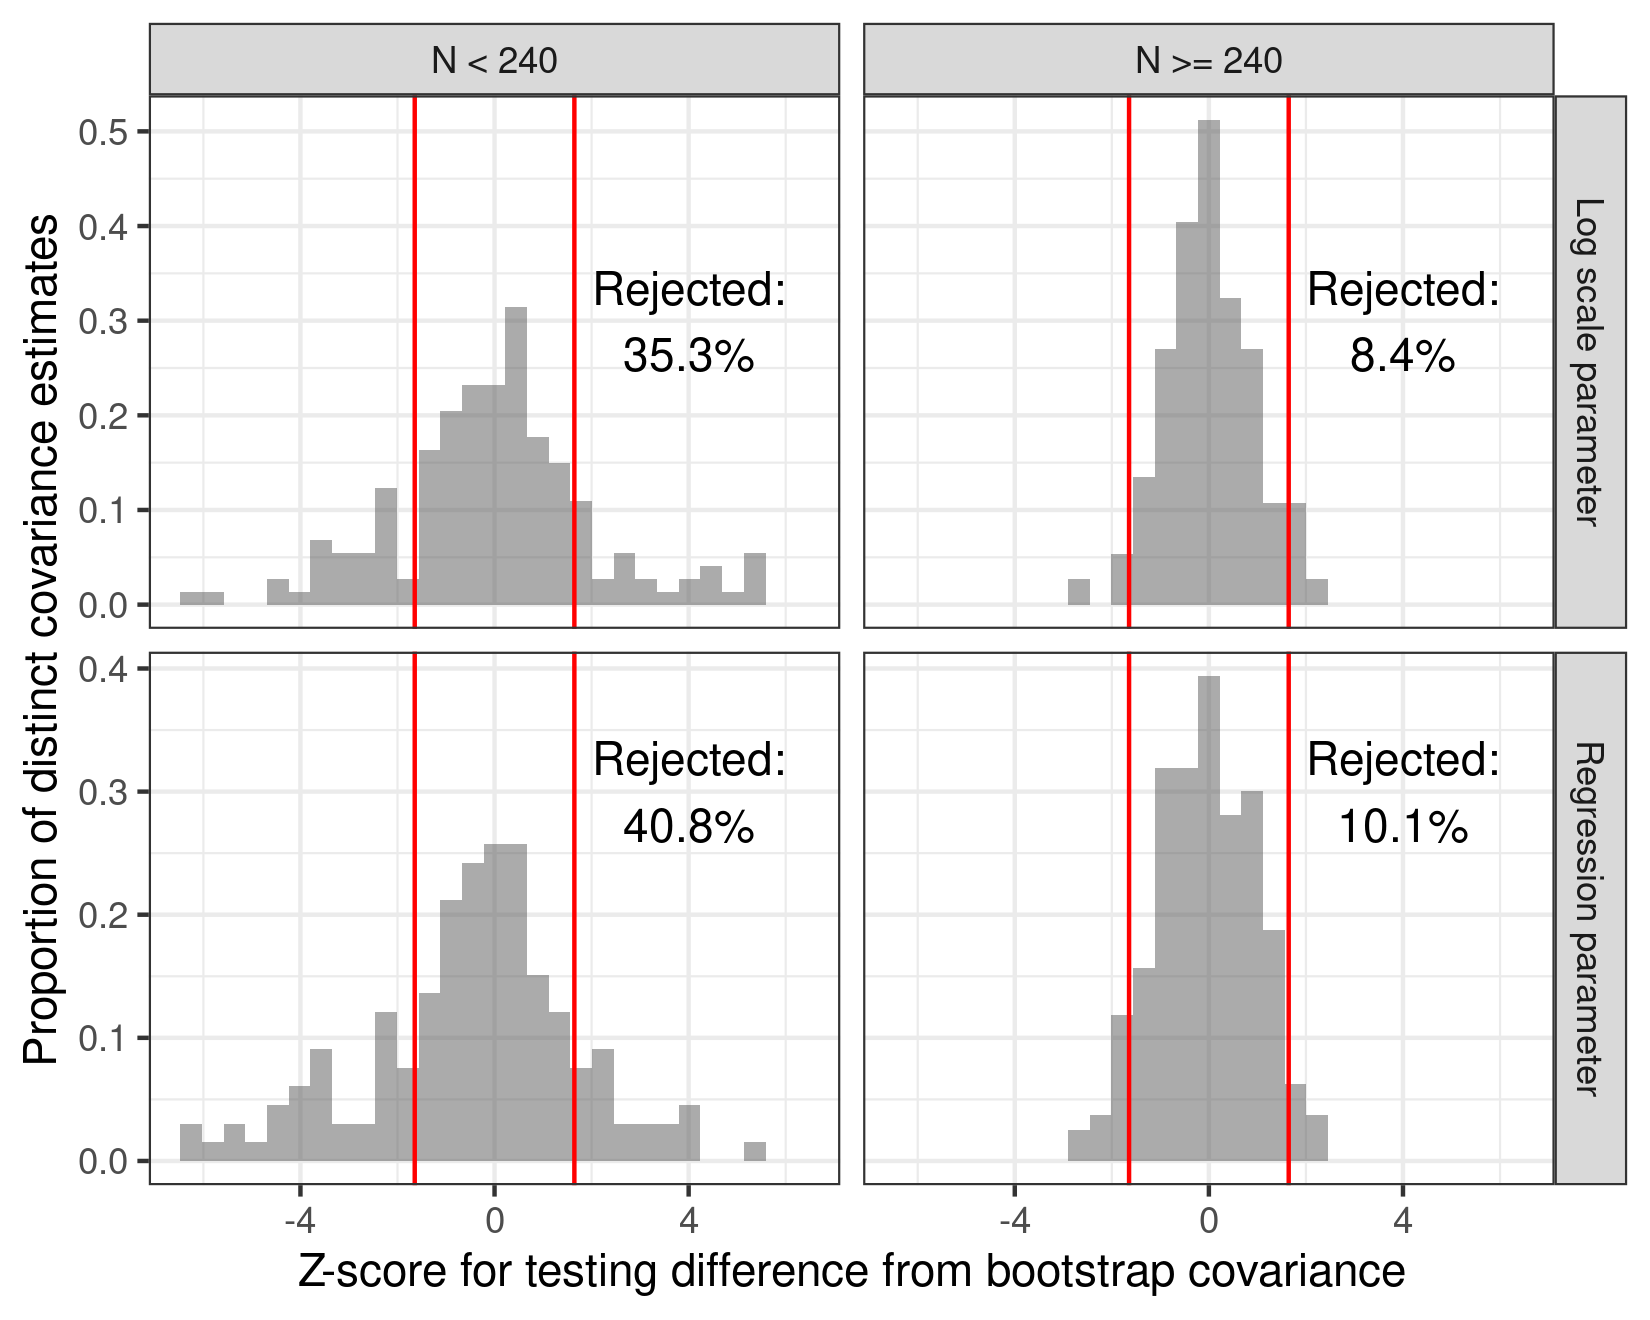
\includegraphics[width=0.98\linewidth,height=0.784\linewidth]{figure/relerr_graph-1} 

}

\caption[The distribution of the z-statistics $\zdiff$]{The distribution of the z-statistics $\zdiff$.  Red lines indicate the boundaries of a normal test for significance with level $0.1$, and ``Rejected'' counts the number of covariances in the rejection region.  Log scale parameters include all variances or covariances that involve at least one log scale parameters.}\label{fig:relerr_graph}
\end{figure}

\end{knitrout}
}


\def\ARMGraphDiff{
%

\begin{knitrout}
\definecolor{shadecolor}{rgb}{0.969, 0.969, 0.969}\color{fgcolor}\begin{figure}[!h]

{\centering 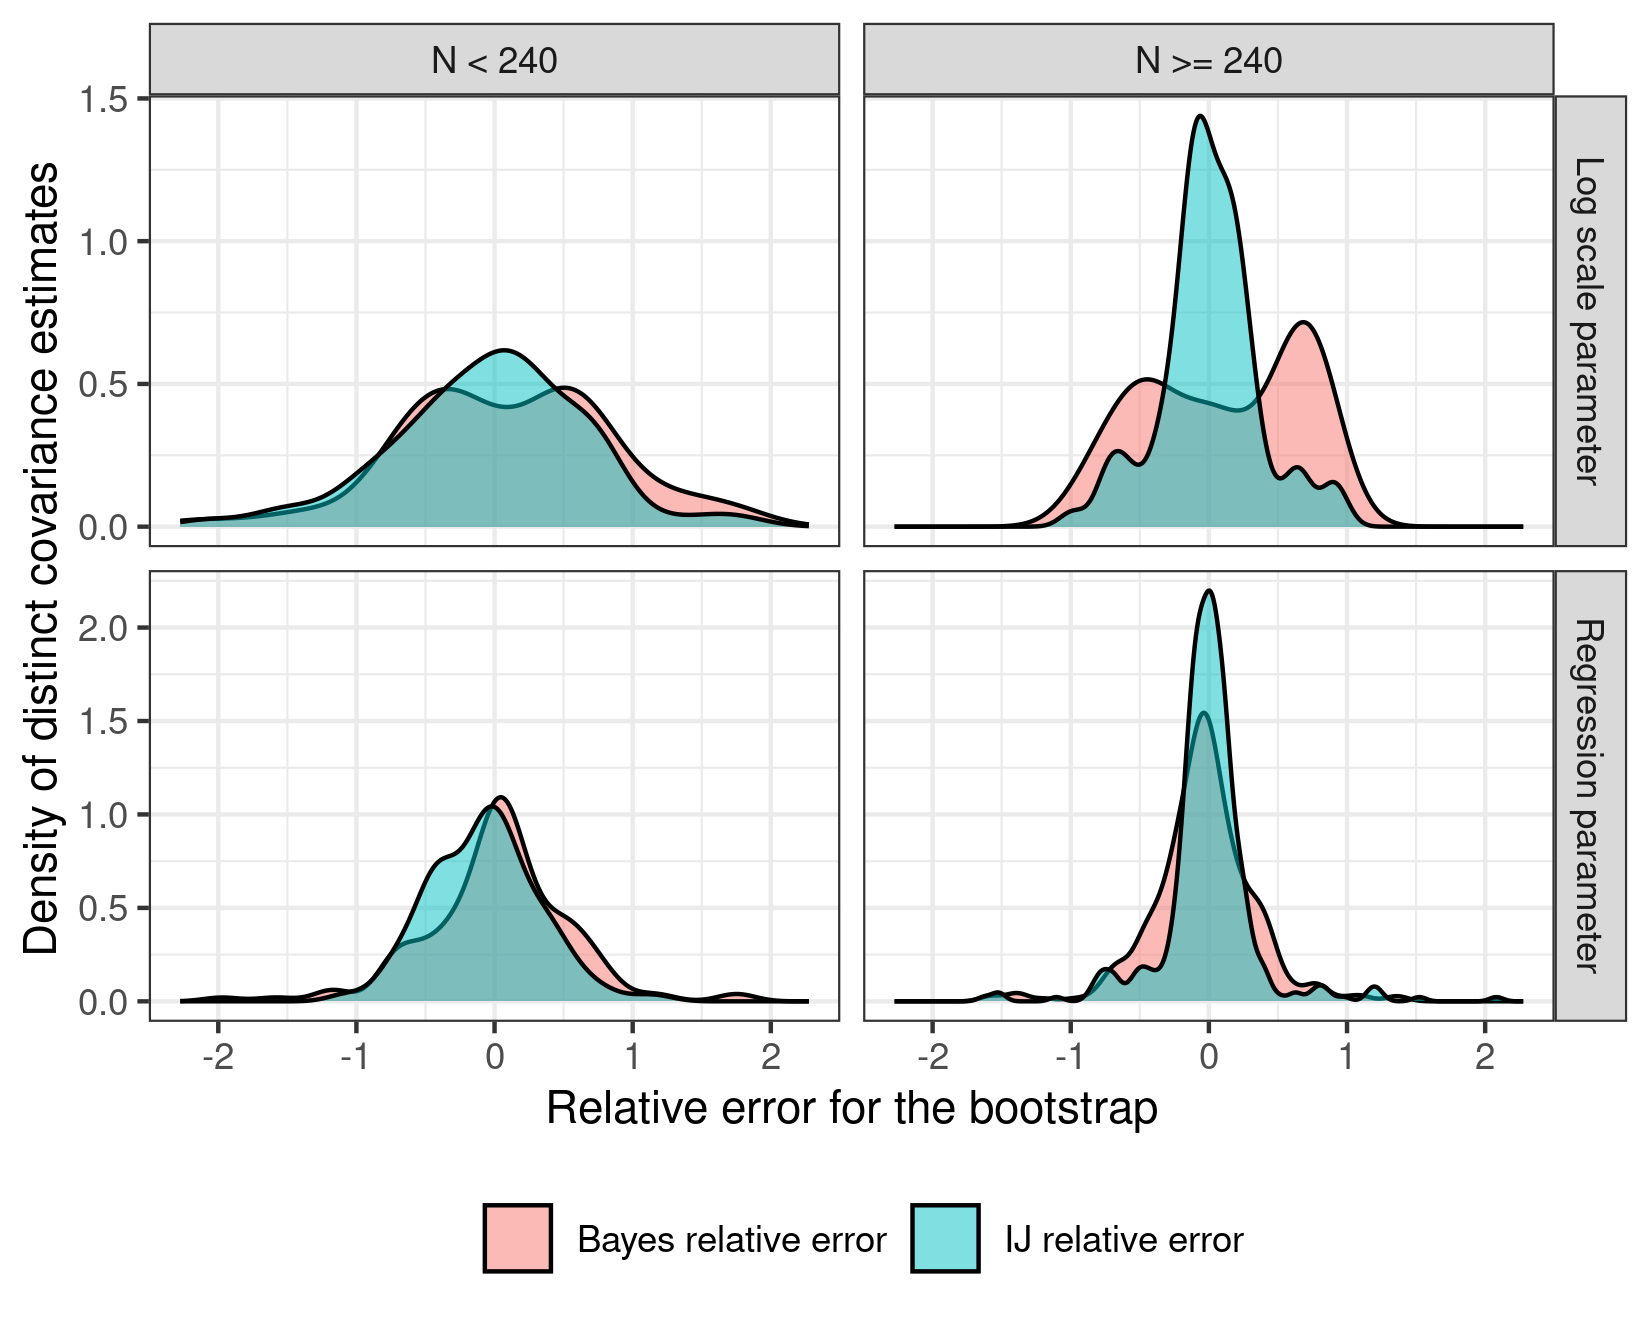
\includegraphics[width=0.98\linewidth,height=0.784\linewidth]{figure/normerr_graph-1} 

}

\caption[The distribution of the relative errors]{The distribution of the relative errors.  Log scale parameters include all variances or covariances that involve at least one log scale parameters.}\label{fig:normerr_graph}
\end{figure}

\end{knitrout}
}

%%%%%%%%%%%%%%%%%%%%%%%%%%%%%%%%%%%%%%%%%%%%%%%%%%%%%%%%%%%%%%%%%%%%%%%%%
%%%%%%%%%%%%%%%%%%%%%%%%%%%%%%%%%%%%%%%%%%%%%%%%%%%%%%%%%%%%%%%%%%%%%%%%%
%%%%%%%%%%%%%%%%%%%%%%%%%%%%%%%%%%%%%%%%%%%%%%%%%%%%%%%%%%%%%%%%%%%%%%%%%

\def\PilotsIntervalsGraph{

\begin{knitrout}
\definecolor{shadecolor}{rgb}{0.969, 0.969, 0.969}\color{fgcolor}\begin{figure}[!h]

{\centering 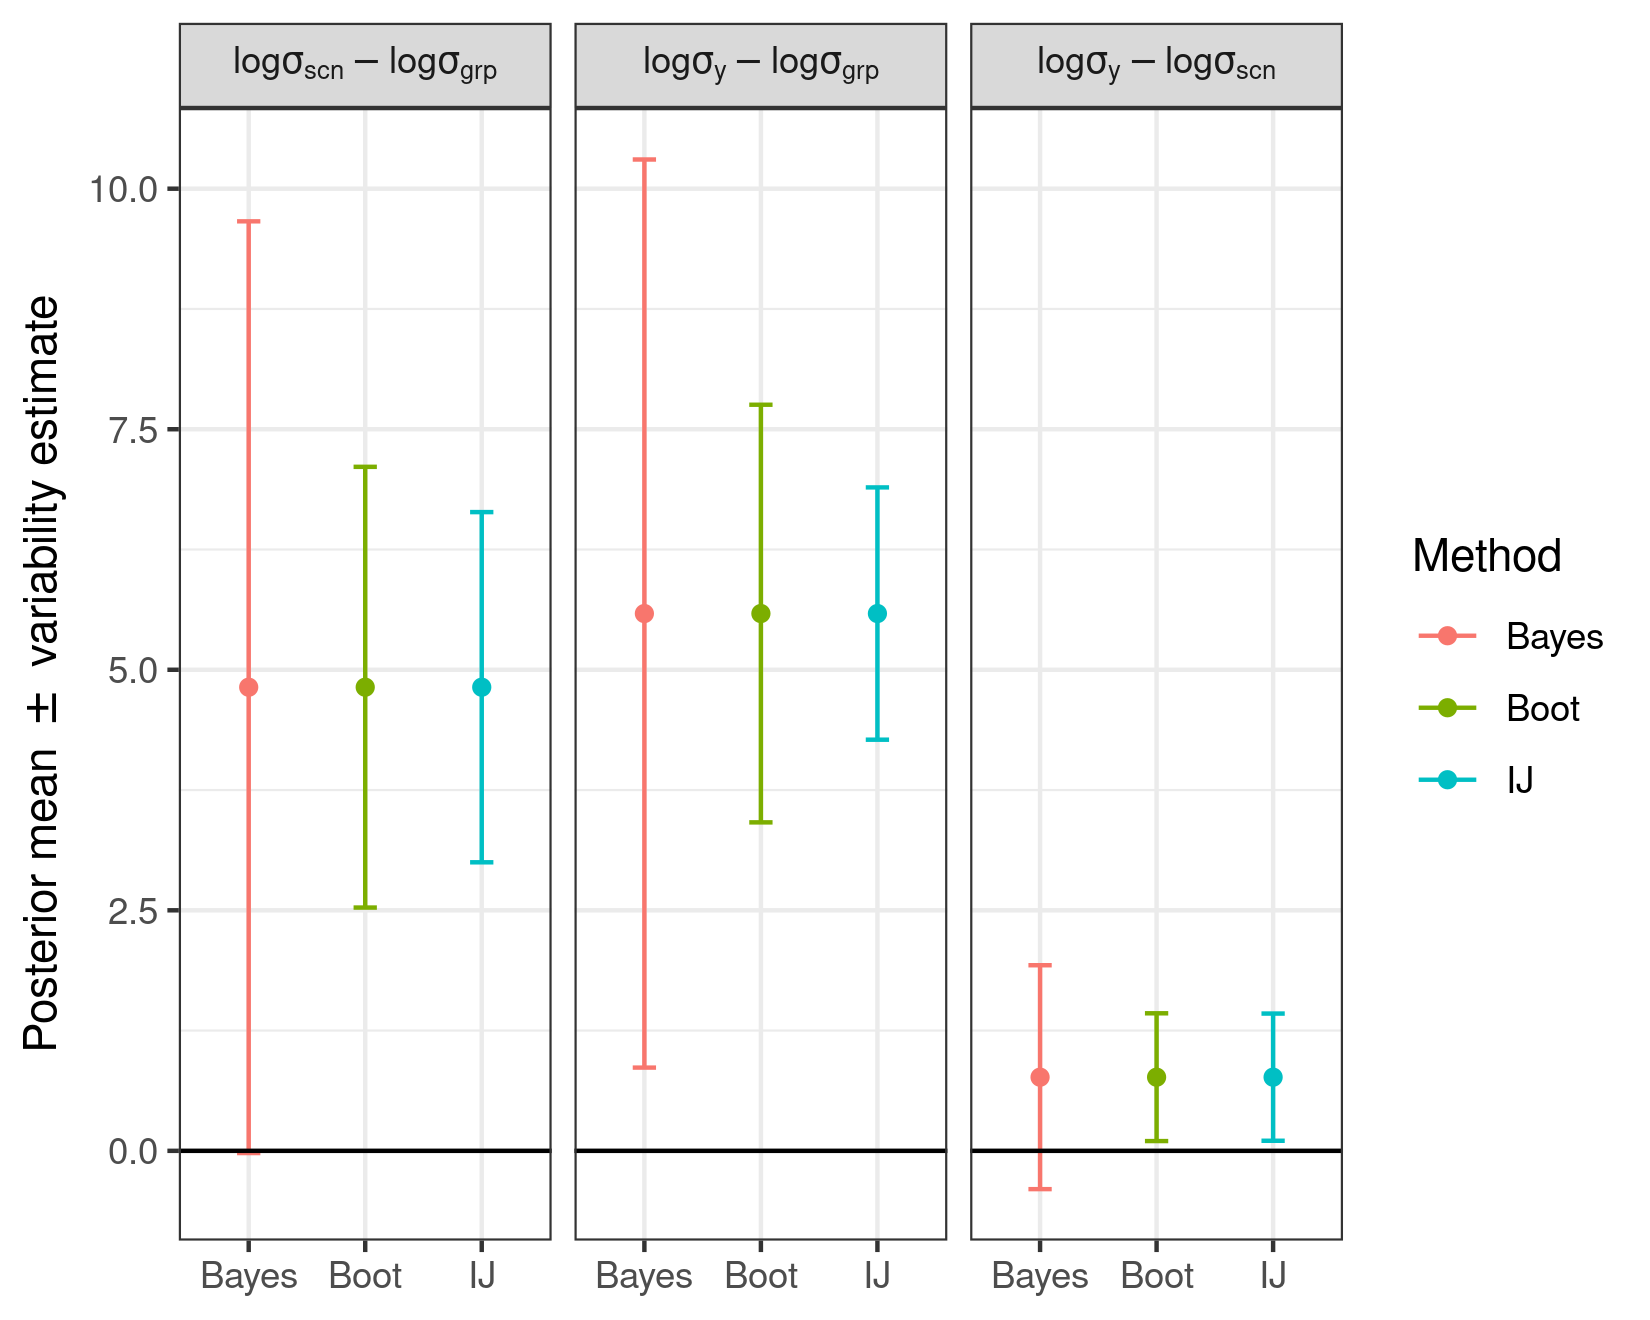
\includegraphics[width=0.98\linewidth,height=0.784\linewidth]{figure/interval_graph-1} 

}

\caption[Means and standard errors for the pilots data]{Means and standard errors for the pilots data. Note that one may make different decisions about the evidence when using the frequentist versus the Bayesian credible intervals, particularly in the first panel.}\label{fig:interval_graph}
\end{figure}

\end{knitrout}
}


\def\PilotsSEGraph{

\begin{knitrout}
\definecolor{shadecolor}{rgb}{0.969, 0.969, 0.969}\color{fgcolor}\begin{figure}[!h]

{\centering 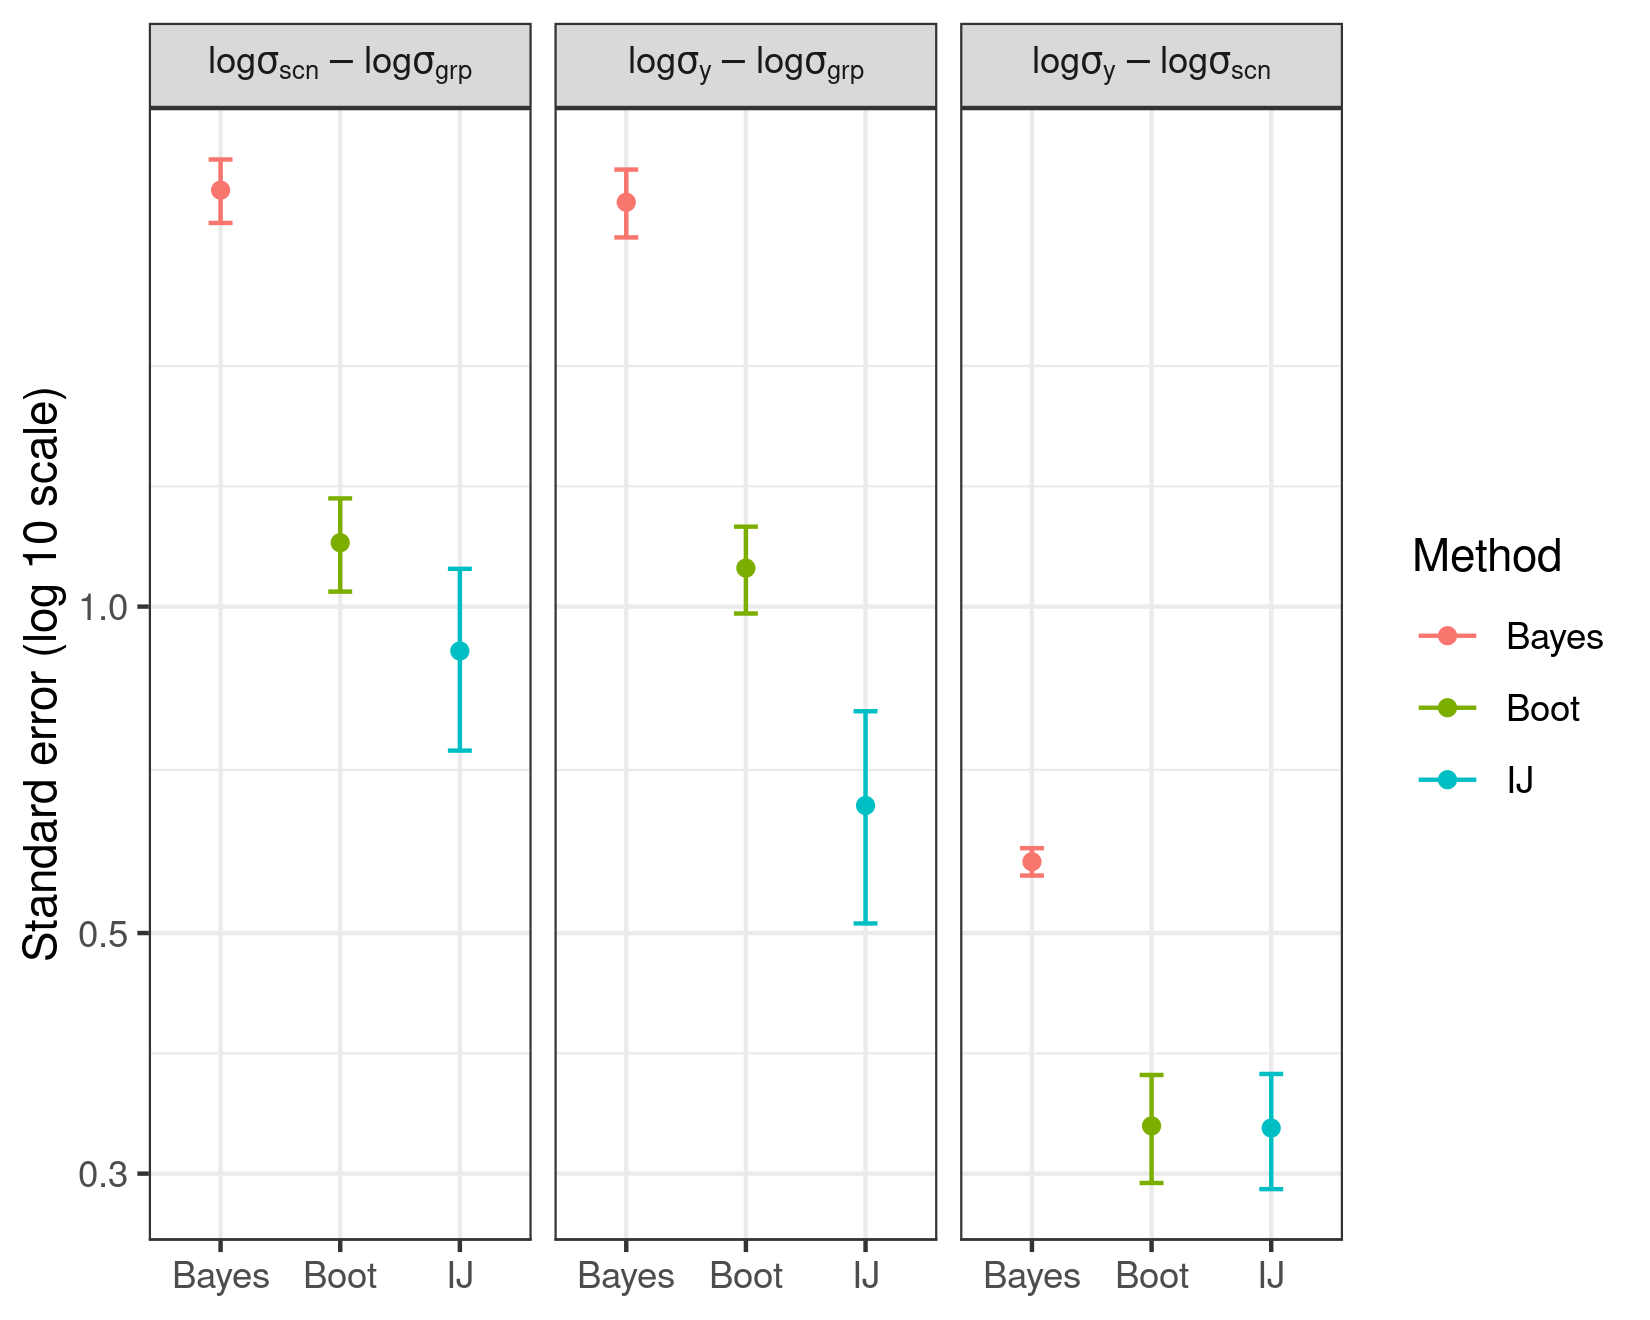
\includegraphics[width=0.98\linewidth,height=0.784\linewidth]{figure/width_graph-1} 

}

\caption[Standard errors (square root of variance estimates / $N$) for the pilots data]{Standard errors (square root of variance estimates / $N$) for the pilots data.}\label{fig:width_graph}
\end{figure}

\end{knitrout}
}


%%%%%%%%%%%%%%%%%%%%%%%%%%%%%%%%%%%%%%%%%%%%%%%%%%%%%%%%%%%%%%%%%%%%%%%%%
%%%%%%%%%%%%%%%%%%%%%%%%%%%%%%%%%%%%%%%%%%%%%%%%%%%%%%%%%%%%%%%%%%%%%%%%%
%%%%%%%%%%%%%%%%%%%%%%%%%%%%%%%%%%%%%%%%%%%%%%%%%%%%%%%%%%%%%%%%%%%%%%%%%


\def\BatsData{

\begin{knitrout}
\definecolor{shadecolor}{rgb}{0.969, 0.969, 0.969}\color{fgcolor}\begin{figure}[!h]

{\centering 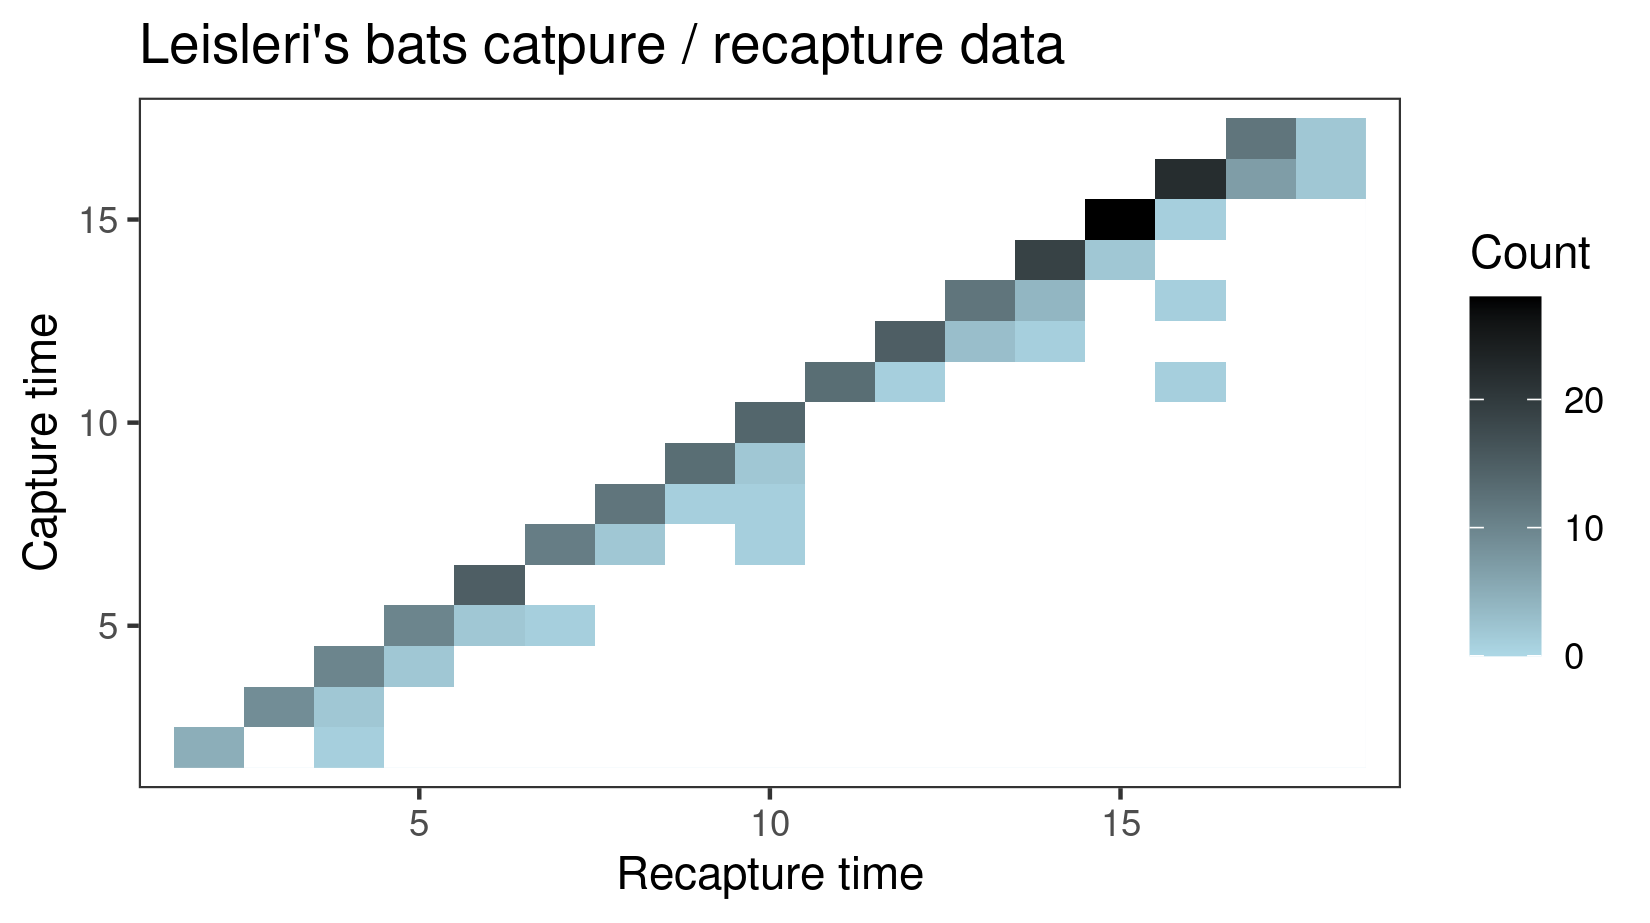
\includegraphics[width=0.98\linewidth,height=0.549\linewidth]{figure/bats_data-1} 

}

\caption[The ragged array counting the number of bats at re-observed a certain number of time periods after each time period]{The ragged array counting the number of bats at re-observed a certain number of time periods after each time period.}\label{fig:bats_data}
\end{figure}

\end{knitrout}
%
}



\def\BatsResults{

\begin{knitrout}
\definecolor{shadecolor}{rgb}{0.969, 0.969, 0.969}\color{fgcolor}\begin{figure}[!h]

{\centering 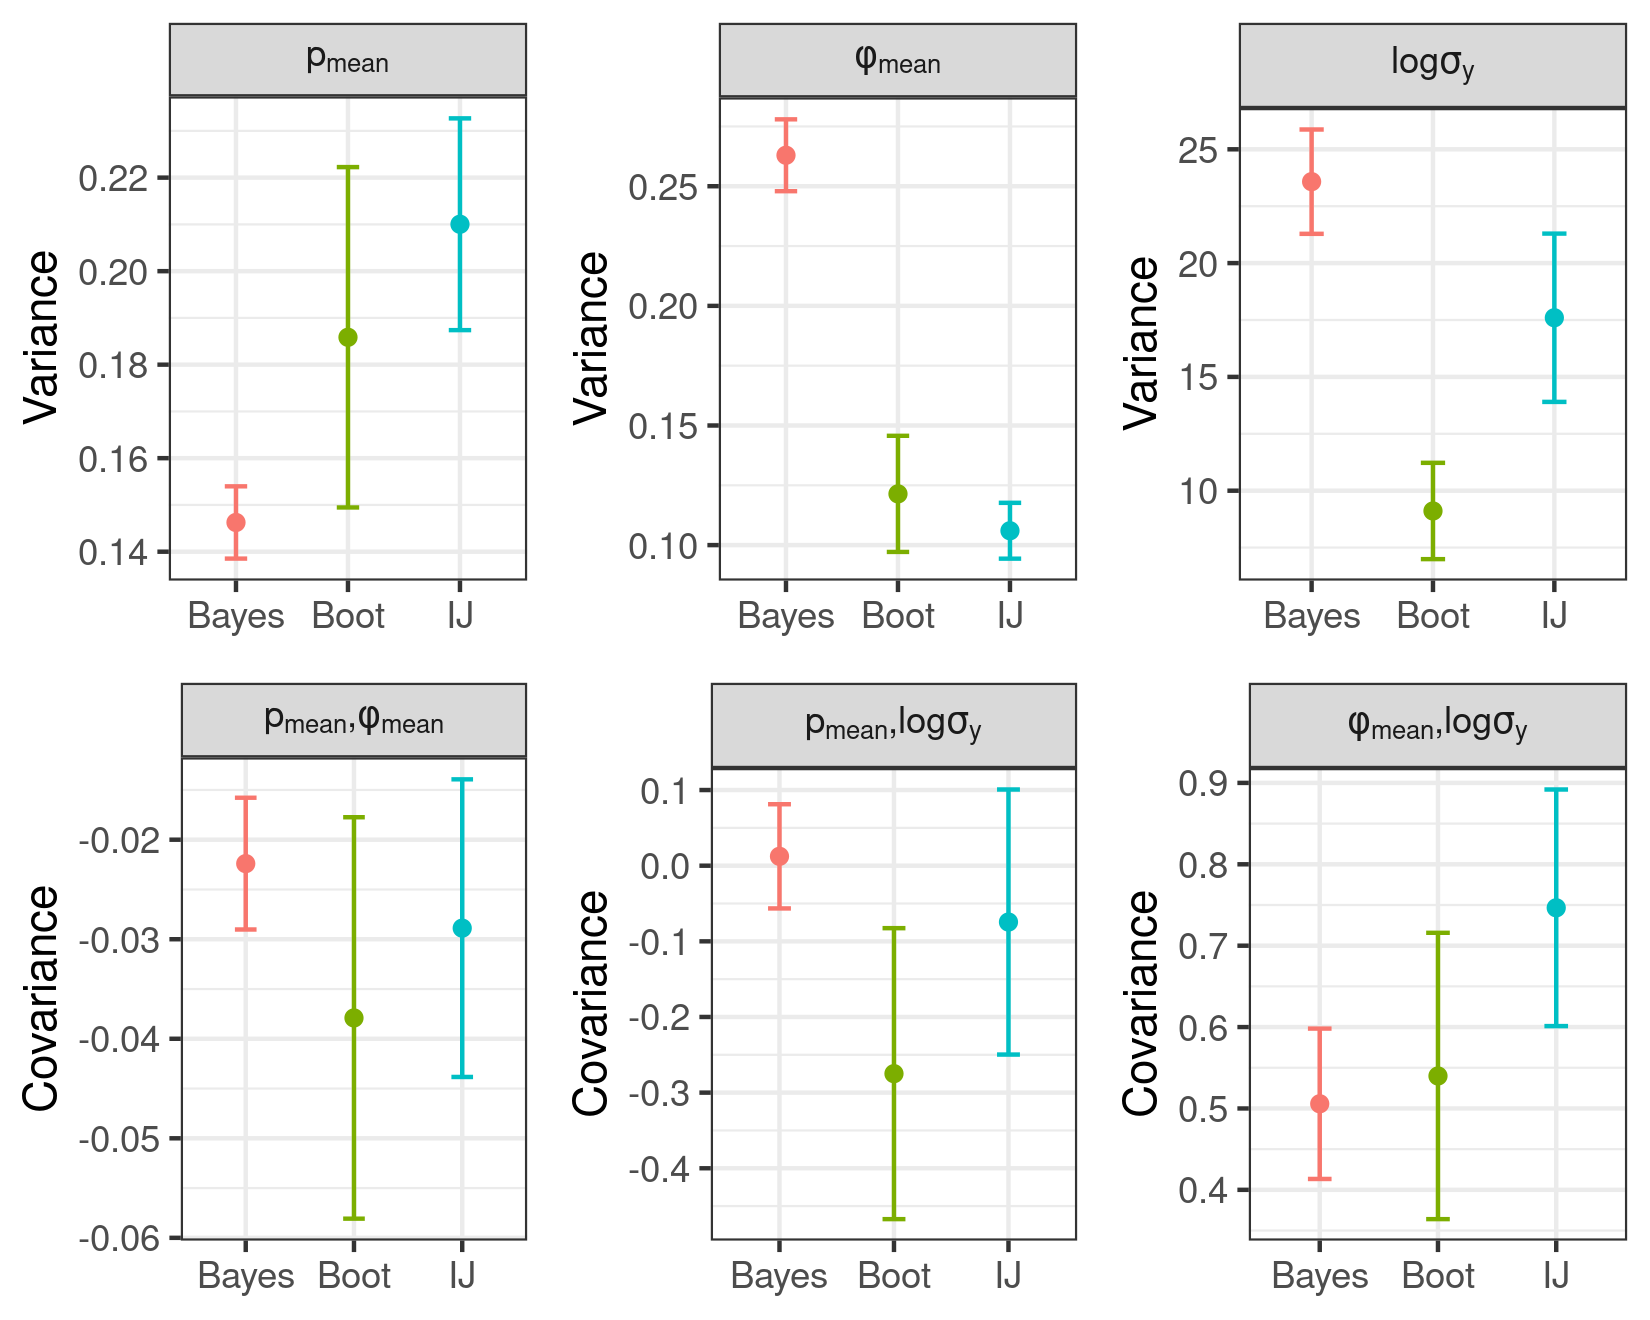
\includegraphics[width=0.98\linewidth,height=0.784\linewidth]{figure/bats_result-1} 

}

\caption[Comparison between $\gcovbayeshat$, $\gcovijhat$, and $\gcovboothat$ for the Leisleri Bats dataset]{Comparison between $\gcovbayeshat$, $\gcovijhat$, and $\gcovboothat$ for the Leisleri Bats dataset.  The first row shows the diagonal entries (variances), and the second row shows the off-diagonal entries (covariances).  Error bars are $2 \sebayes$, $2 \seij$, and $2 \seboot$, respectively.  Note that the scales of the y axes are all different to allow for joint plotting.}\label{fig:bats_result}
\end{figure}

\end{knitrout}
%
}


%%%%%%%%%%%%%%%%%%%%%%%%%%%%%%%%%%%%%%%%%%%%%%%%%%%%%%%%%%%%%%%%%%%%%%%%%
%%%%%%%%%%%%%%%%%%%%%%%%%%%%%%%%%%%%%%%%%%%%%%%%%%%%%%%%%%%%%%%%%%%%%%%%%
%%%%%%%%%%%%%%%%%%%%%%%%%%%%%%%%%%%%%%%%%%%%%%%%%%%%%%%%%%%%%%%%%%%%%%%%%


% Broken --- missing predictions dataframe
% \def\POTUSData{
% <<graph_fig_cap7>>=
% figcap <- paste(
%     "Some real data. ",
%     "of the IJ and simulation, frequentist error.",
%     sep="")
% SetShortImageSize()
% @
% <<election_data, cache=cache_potus, fig.show='hold', fig.cap=figcap>>=
% source("R_scripts/election/data_graph.R",
%        echo=knitr_debug, print.eval=TRUE)
% @
% }


\def\POTUSStatesGraph{


\begin{knitrout}
\definecolor{shadecolor}{rgb}{0.969, 0.969, 0.969}\color{fgcolor}\begin{figure}[!h]

{\centering 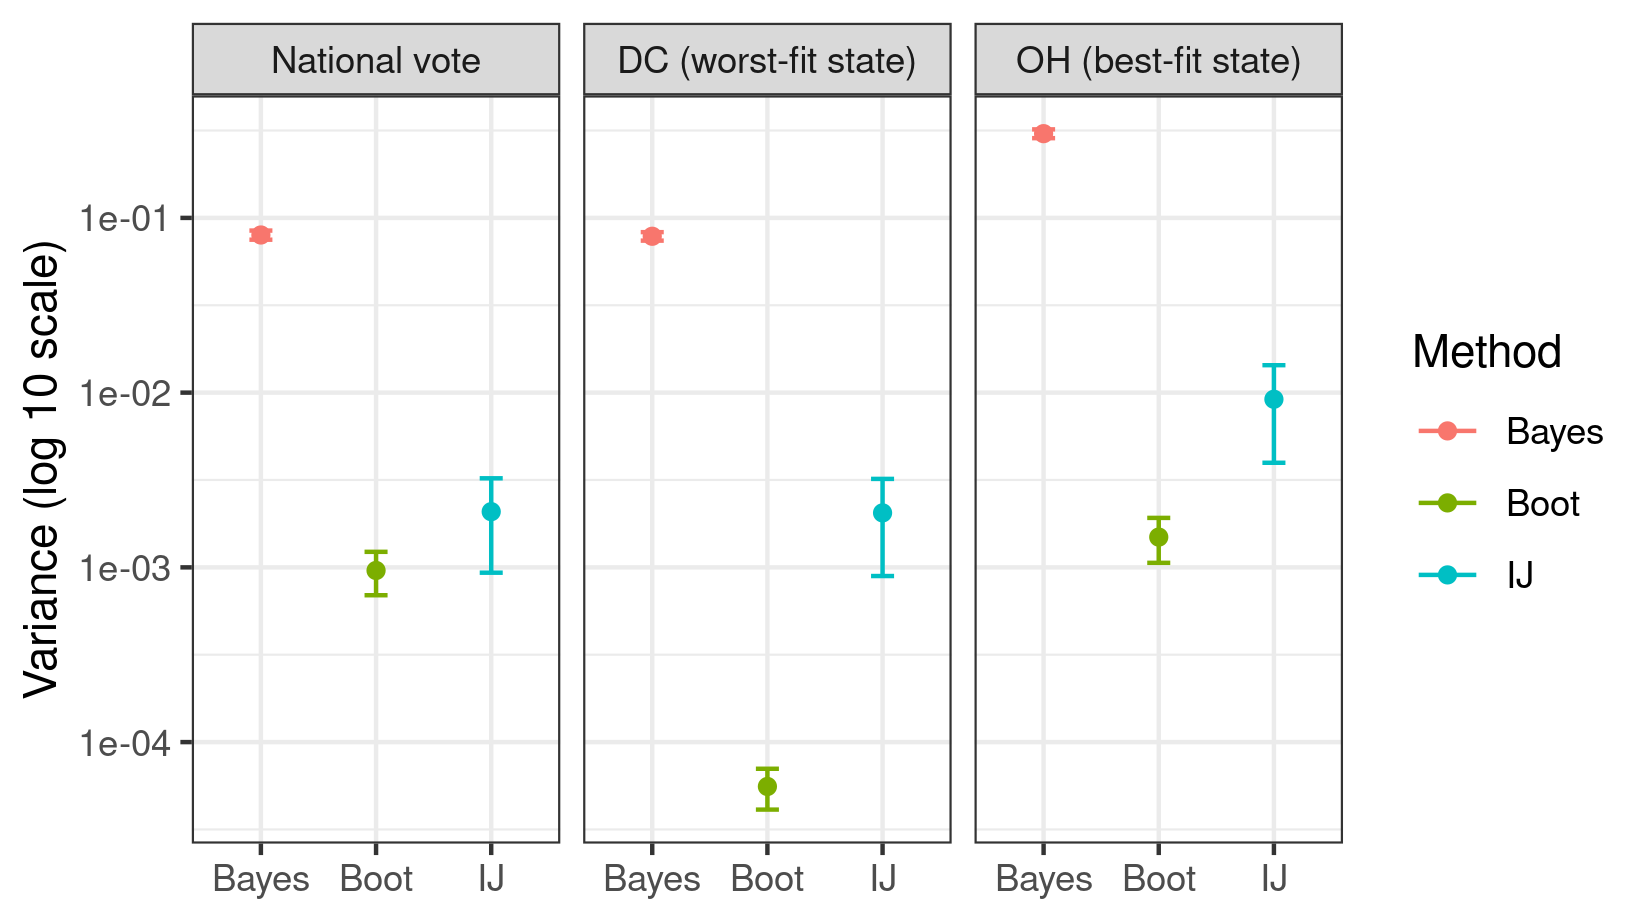
\includegraphics[width=0.98\linewidth,height=0.549\linewidth]{figure/election_result-1} 

}

\caption[Selected for the national vote and the two states in which the IJ performed worst and best]{Selected for the national vote and the two states in which the IJ performed worst and best.  Note the log10 scale of the y-axis.  The upper and lower extent of the error bars were computed using $2 \seij$, $2 \sebayes$, and $2 \seboot$ before transforming by log10 for plotting.}\label{fig:election_result}
\end{figure}

\end{knitrout}
%
}

\def\POTUSScatterGraph{

\begin{knitrout}
\definecolor{shadecolor}{rgb}{0.969, 0.969, 0.969}\color{fgcolor}\begin{figure}[!h]

{\centering 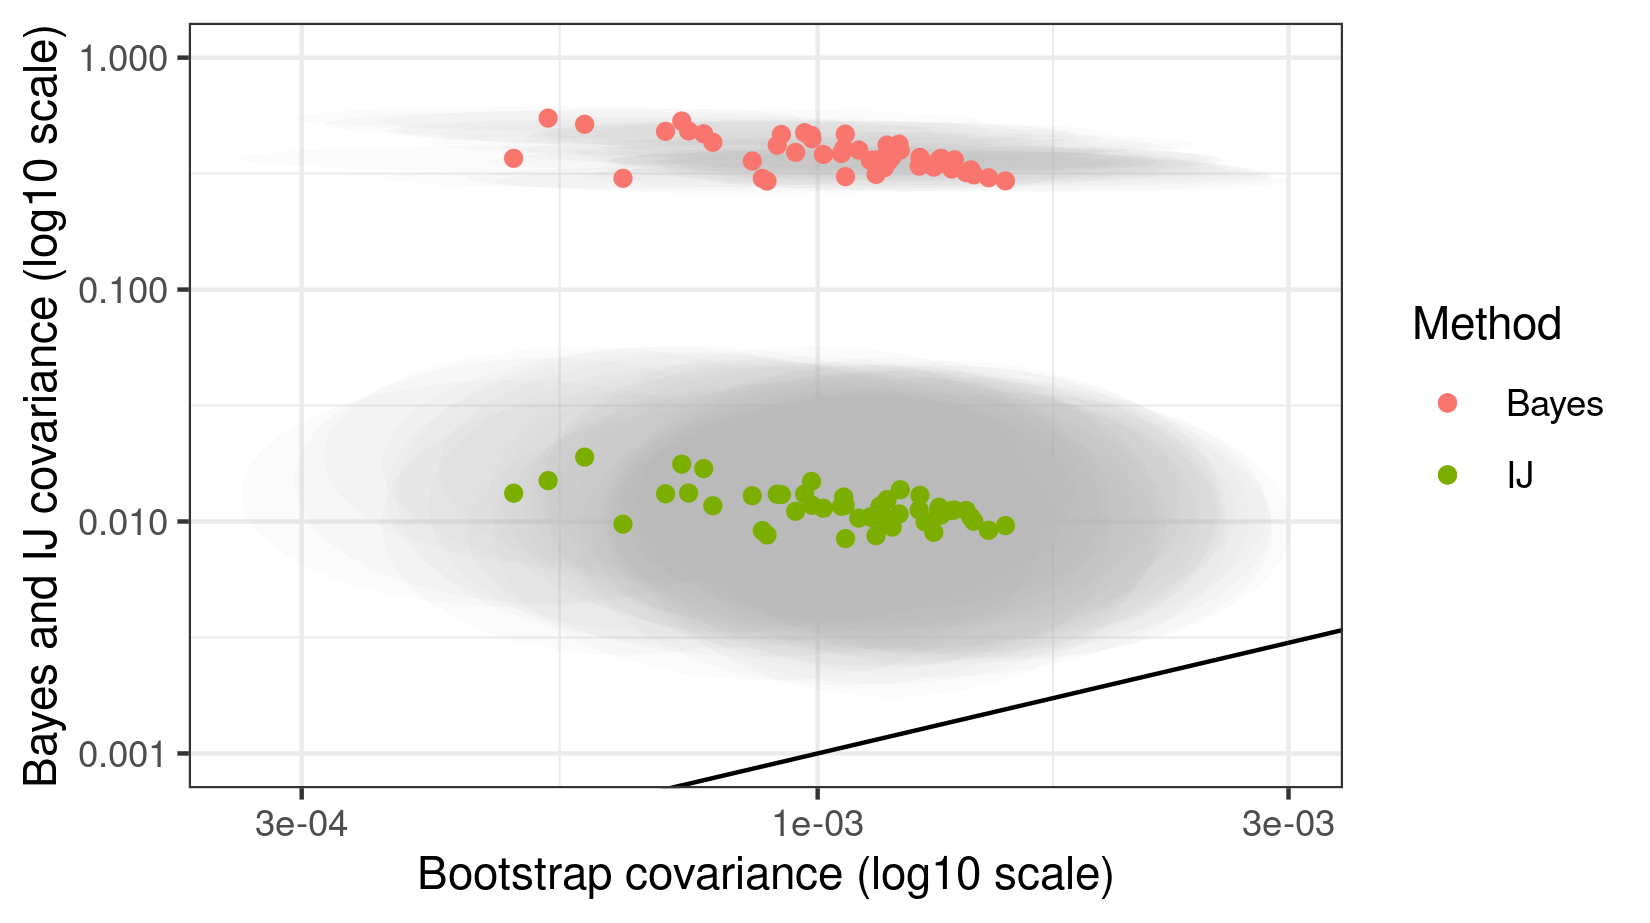
\includegraphics[width=0.98\linewidth,height=0.549\linewidth]{figure/election_state_result-1} 

}

\caption[Scatterplot of the diagonals of $\gcovbayeshat$, $\gcovijhat$, and $\gcovboothat$ for all the states except DC]{Scatterplot of the diagonals of $\gcovbayeshat$, $\gcovijhat$, and $\gcovboothat$ for all the states except DC.  Note the log10 scale of the y-axis.  The extent of the confidence ellipses (shown in gray) were computed using $2 \seij$, $2 \sebayes$, and $2 \seboot$ before transforming by log10 for plotting.}\label{fig:election_state_result}
\end{figure}

\end{knitrout}
%
}




%%%%%%%%%%%%%%%%%%%%%%%%%%%%%%%%%%%%%%%%%%%%%%%%%%%%%%%%%%%%%%%%%%%%%%%%%
%%%%%%%%%%%%%%%%%%%%%%%%%%%%%%%%%%%%%%%%%%%%%%%%%%%%%%%%%%%%%%%%%%%%%%%%%
%%%%%%%%%%%%%%%%%%%%%%%%%%%%%%%%%%%%%%%%%%%%%%%%%%%%%%%%%%%%%%%%%%%%%%%%%

\def\SingularResultsGraph{

\begin{knitrout}
\definecolor{shadecolor}{rgb}{0.969, 0.969, 0.969}\color{fgcolor}\begin{figure}[!h]

{\centering 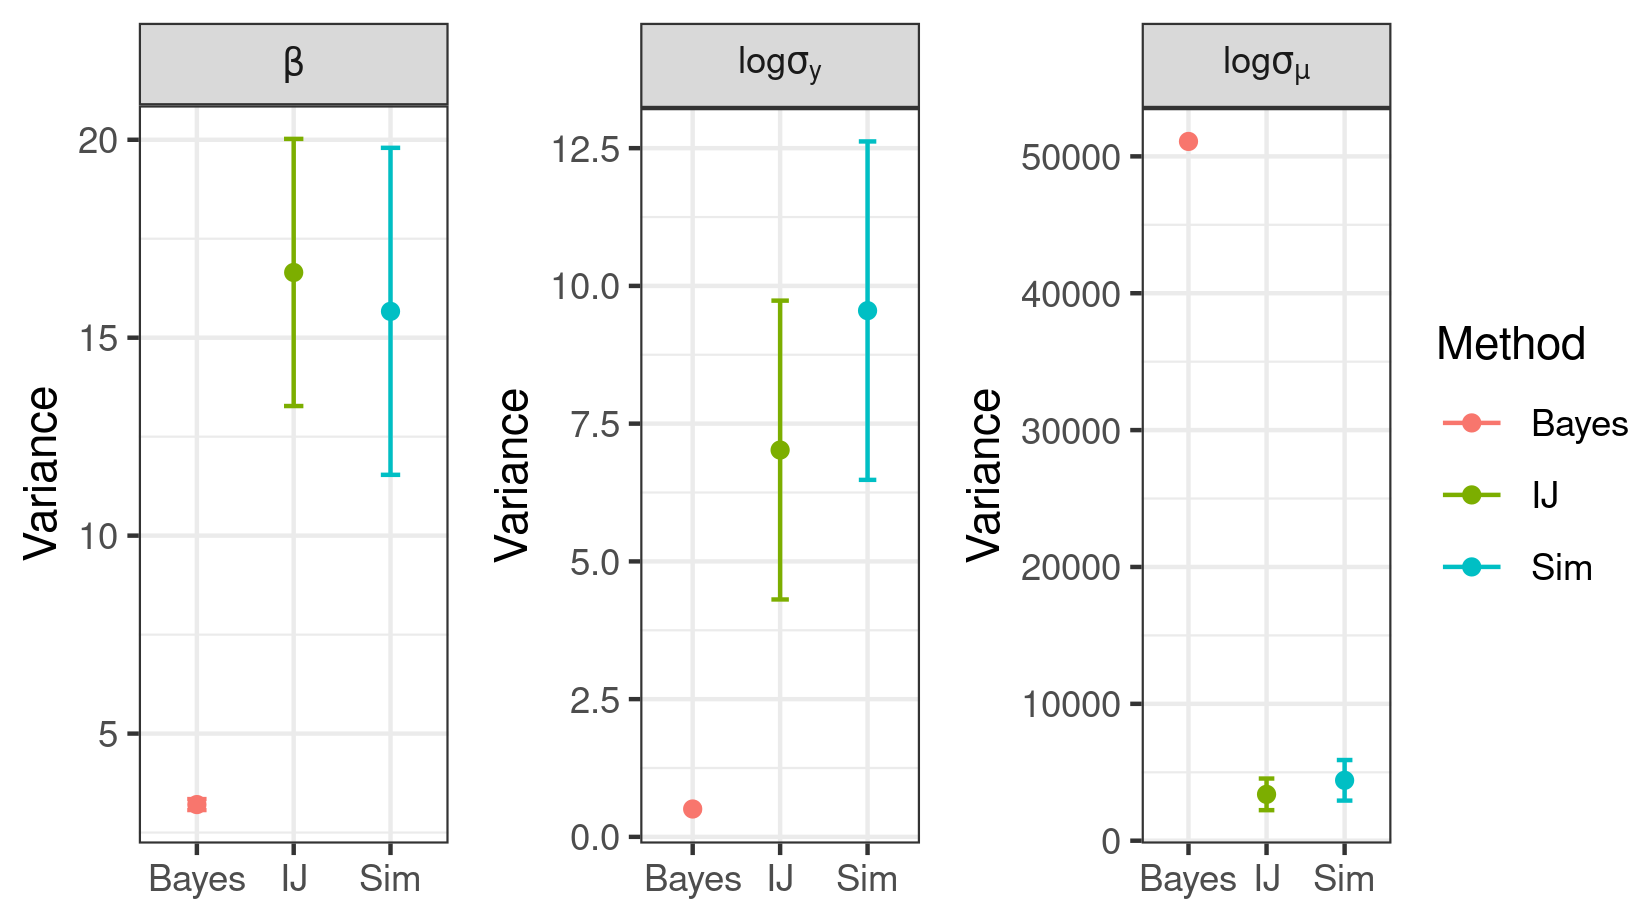
\includegraphics[width=0.98\linewidth,height=0.549\linewidth]{figure/simple_sim_result-1} 

}

\caption[The difference from the simulation, IJ, and Bayesian covariances]{The difference from the simulation, IJ, and Bayesian covariances. Standard include variation due to both Monte Carlo and, in the case of the IJ and simulation, frequentist error.}\label{fig:simple_sim_result}
\end{figure}

\end{knitrout}
%
}


%%%%%%%%%%%%%%%%%%%%%%%%%%%%%%%%%%%%%%%%%%%%%%%%%%%%%%%%%%%%%%%%%%%%%%%%%
%%%%%%%%%%%%%%%%%%%%%%%%%%%%%%%%%%%%%%%%%%%%%%%%%%%%%%%%%%%%%%%%%%%%%%%%%
%%%%%%%%%%%%%%%%%%%%%%%%%%%%%%%%%%%%%%%%%%%%%%%%%%%%%%%%%%%%%%%%%%%%%%%%%
%
% <<sim_ar_vars>>=
% sim_ar <- 1.
% sim_img_over_legend <- 2
% sim_r_width <- 2.7
% @

\newcommand{\PoissonREGraph}{

\begin{knitrout}
\definecolor{shadecolor}{rgb}{0.969, 0.969, 0.969}\color{fgcolor}\begin{figure}[!h]

{\centering 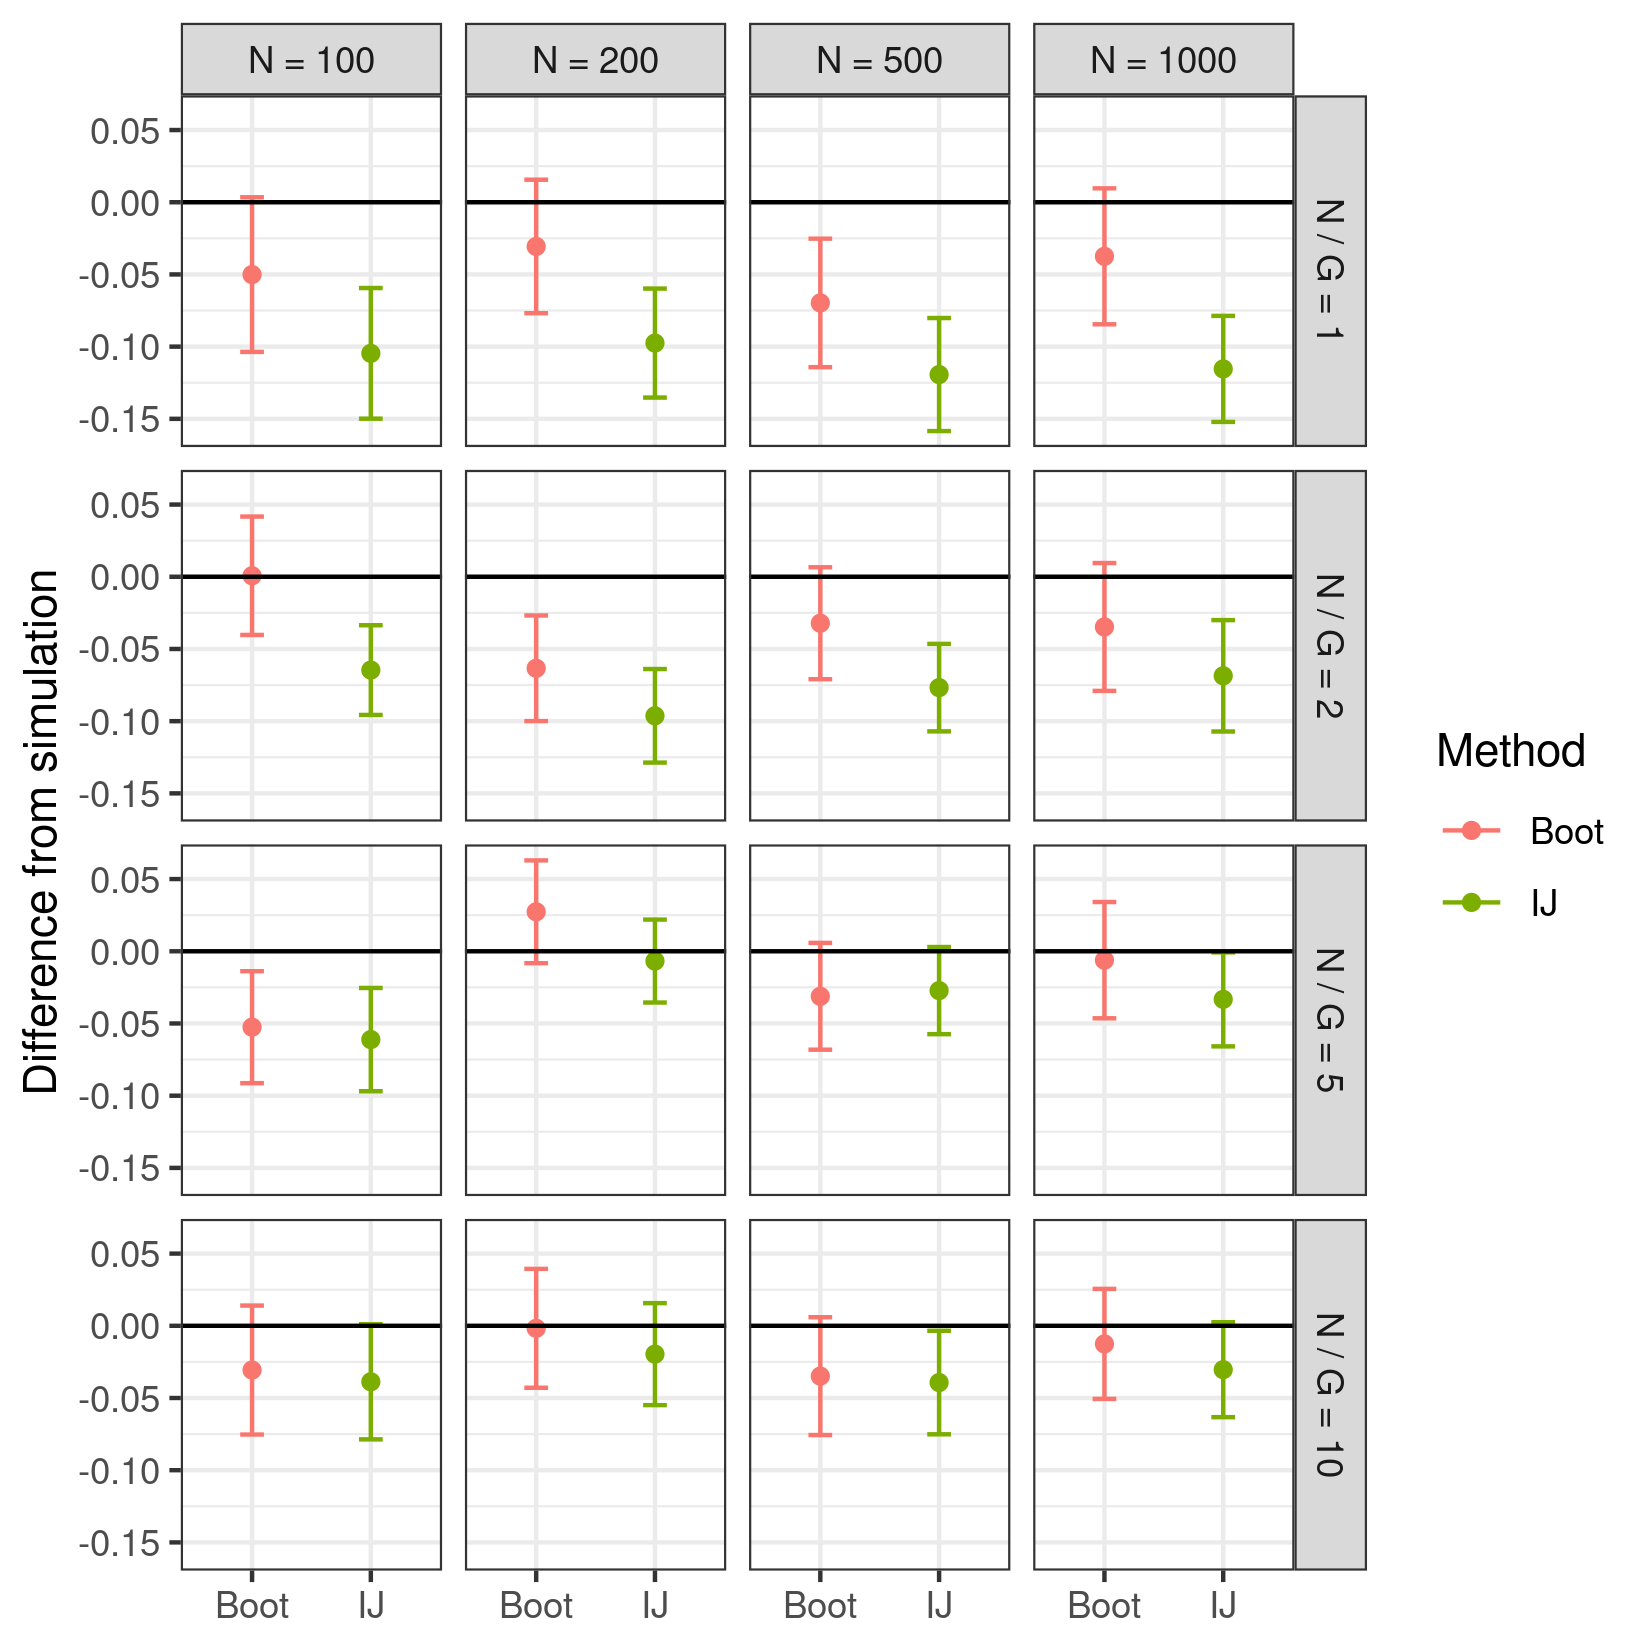
\includegraphics[width=0.98\linewidth,height=0.980\linewidth]{figure/poisson_re_graph-1} 

}

\caption[The error of the IJ and bootstrap covariances for different values of $N$ and $G$]{The error of the IJ and bootstrap covariances for different values of $N$ and $G$.  The y-axis shows the difference between $N (V - \hat{V}_{\mathrm{sim}})$, where $V$ is either $\gcovijhat$ or $\gcovboothat$.}\label{fig:poisson_re_graph}
\end{figure}

\end{knitrout}
}










%%%%%%%%%%%%%%%%%%%%%%%%%%%%%%%%%%%%%%%%%%%%%%%%%%%%%%%%%%%%%%%%%%%%%%%%%
%%%%%%%%%%%%%%%%%%%%%%%%%%%%%%%%%%%%%%%%%%%%%%%%%%%%%%%%%%%%%%%%%%%%%%%%%
%%%%%%%%%%%%%%%%%%%%%%%%%%%%%%%%%%%%%%%%%%%%%%%%%%%%%%%%%%%%%%%%%%%%%%%%%
% Presentation graphs


% \newcommand{\LowDimAccuracyGraph}{
% %<<mult_path, cache=cache, fig.show='hold', fig.cap=fig_cap>>=
% <<lowdim_accuracy, cache=knitr_cache, fig.show='hold'>>=

% bclt_df <- df %>%
%     filter(!as.logical(is_cond), num_obs == num_g)

% num_obs <- 800
% ggplot(bclt_df %>% filter(num_obs == !!num_obs)) +
%     geom_point(aes(x=diff_refit, diff_pred)) +
%     geom_abline(aes(slope=1, intercept=0)) +
%     xlab(TeX("Actual difference in $E\\[\\gamma | X\\]$")) +
%     ylab(TeX("Linear approximation")) +
%     ggtitle(sprintf(paste0(
%         "Negative Binomial model \n",
%         "leaving out single datapoints with N = %d"
%         ), num_obs))
% @
% }



% \newcommand{\HighDimAccuracyGraph}{
% %<<mult_path, cache=cache, fig.show='hold', fig.cap=fig_cap>>=
% <<highdim_accuracy, cache=knitr_cache, fig.show='hold'>>=

% nonbclt_df <- df %>%
%     filter(as.logical(is_cond), num_obs == num_g)

% num_obs <- 800
% ggplot(nonbclt_df %>% filter(num_obs == !!num_obs)) +
%     geom_point(aes(x=diff_refit, diff_pred)) +
%     geom_abline(aes(slope=1, intercept=0)) +
%     xlab(TeX("Actual difference in $E\\[\\gamma | X\\]$")) +
%     ylab(TeX("Linear approximation")) +
%     ggtitle(sprintf(paste0(
%         "Poisson random effect model \n",
%         "leaving out single datapoints with N = %d"
%         ), num_obs))
% @
% }



% \newcommand{\ElectionResultsGlobal}{
% <<graph_fig_cap2_presentation>>=
% SetSlideImageSize(aspect_ratio=1.2, width=0.98)
% @
% <<election_result_presentation, cache=knitr_cache, fig.show='hold'>>=
% source(file.path(r_script_dir, "election/result_national_graph.R"),
%        echo=knitr_debug, print.eval=TRUE)
% @
% }
